


%!TEX program = xelatex
\documentclass[xcolor={table}]{beamer}

% Packages
\usepackage[brazil]{babel}	
\usepackage[utf8]{inputenc}
\usepackage[T1]{fontenc}
\usepackage[scaled]{helvet}
\usepackage{amsthm}
\usepackage{ragged2e}
\usepackage{subfig}
\usepackage[table]{xcolor}
\usepackage{multicol}
\usepackage{multirow}
\usepackage{fancyvrb}
\usepackage{verbatim}
\usepackage{minted}

% Configuration for packages
\usemintedstyle{bw}

% Theme
\usetheme{Execushares}

% Title page
\title{Naevia}
\author{%
    Apostolescu Ștefan \\
    Băjan Ionuț-Mihăiță \\
    Iosif George-Andrei
}
\setcounter{showSlideNumbers}{1}

\begin{document}

    % Title page
    \setcounter{showProgressBar}{0}
	\setcounter{showSlideNumbers}{0}
	\frame{\titlepage}

    % Table of content
	\begin{frame}
		\large{\frametitle{Tabelă de Conținut}}
		\begin{enumerate}
			\item Detalii despre Aplicație
			\item Noțiuni Teoretice
			\item \textit{Hill Climbing} pentru Criptanaliză
			\item Arhitectura Aplicației
			\item Demonstrație
		\end{enumerate}
	\end{frame}

	\setcounter{framenumber}{0}
	\setcounter{showProgressBar}{1}
	\setcounter{showSlideNumbers}{1}

	\begin{frame}
		\frametitle{Detalii despre Aplicație} \pause
		\begin{itemize}
			\item \textbf{Naevia} este dezvoltată ca temă pentru cursul de "\textit{Inteligență Artificială}". \pause
			\item Obiectivele propuse țin de: \pause
			    \begin{enumerate}
                    \item folosirea tehnicii \textit{Hill Climbing} pentru optimizarea procesului de criptanaliza a unor cifruri clasice; \pause
                    \item criptarea textelor cu ajutorul cifrurilor implementate; și de \pause
                    \item compararea abordarii bazate pe forță brută cu cea optimizată, prin intermediul graficelor.
                \end{enumerate}
		\end{itemize}
	\end{frame}
	
	\begin{frame}
		\frametitle{Noțiuni Teoretice} \pause
		\begin{itemize}
			\item Cifruri Clasice \pause
			    \begin{itemize}
			        \item Caesar \pause
			        \item Vigenère \pause
			        \item de substituție \pause
			    \end{itemize}
			\item \textit{Hill Climbing}
		\end{itemize}
	\end{frame}
	
	\begin{frame}
		\frametitle{\textit{Hill Climbing} pentru Criptanaliză} \pause
		\begin{itemize}
			\item mod generic de funcționare \pause
			\item funcția de generare de stări \pause
			\item funcția euristică
		\end{itemize}
	\end{frame}
	
	\begin{frame}
		\frametitle{Arhitectura Aplicației} \pause
		\begin{center}
            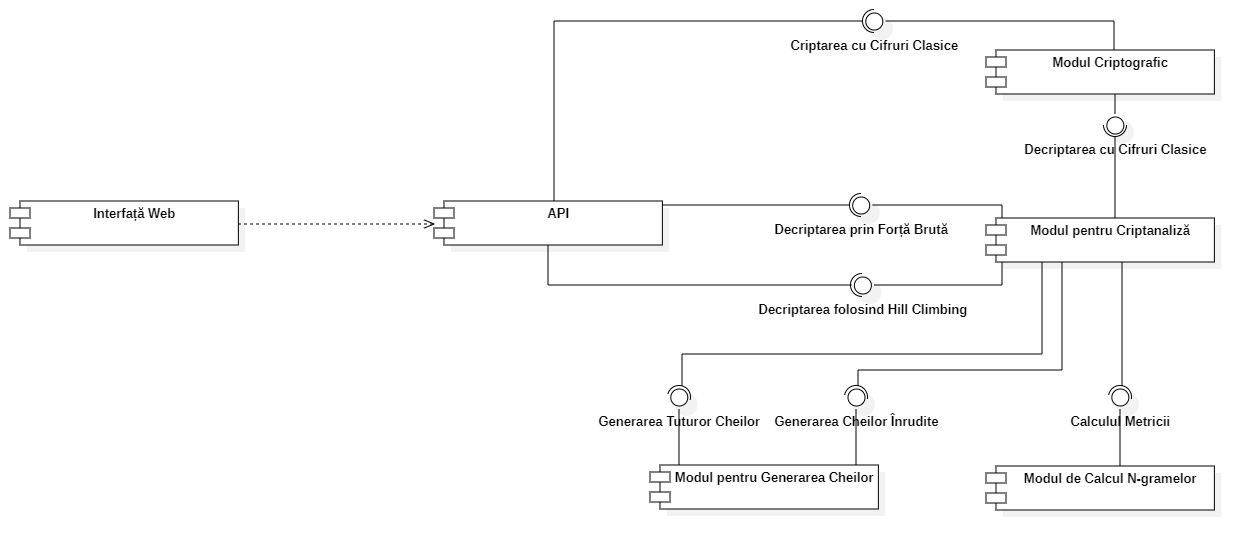
\includegraphics[width=9cm]{images/components_diagram.png}
            \label{fig:infrastructure}
        \end{center}
	\end{frame}

	\section{Demonstrație}

\end{document}